

\subsubsection{Obsługa klienta}

	\begin{figure}[H]
		\centering
		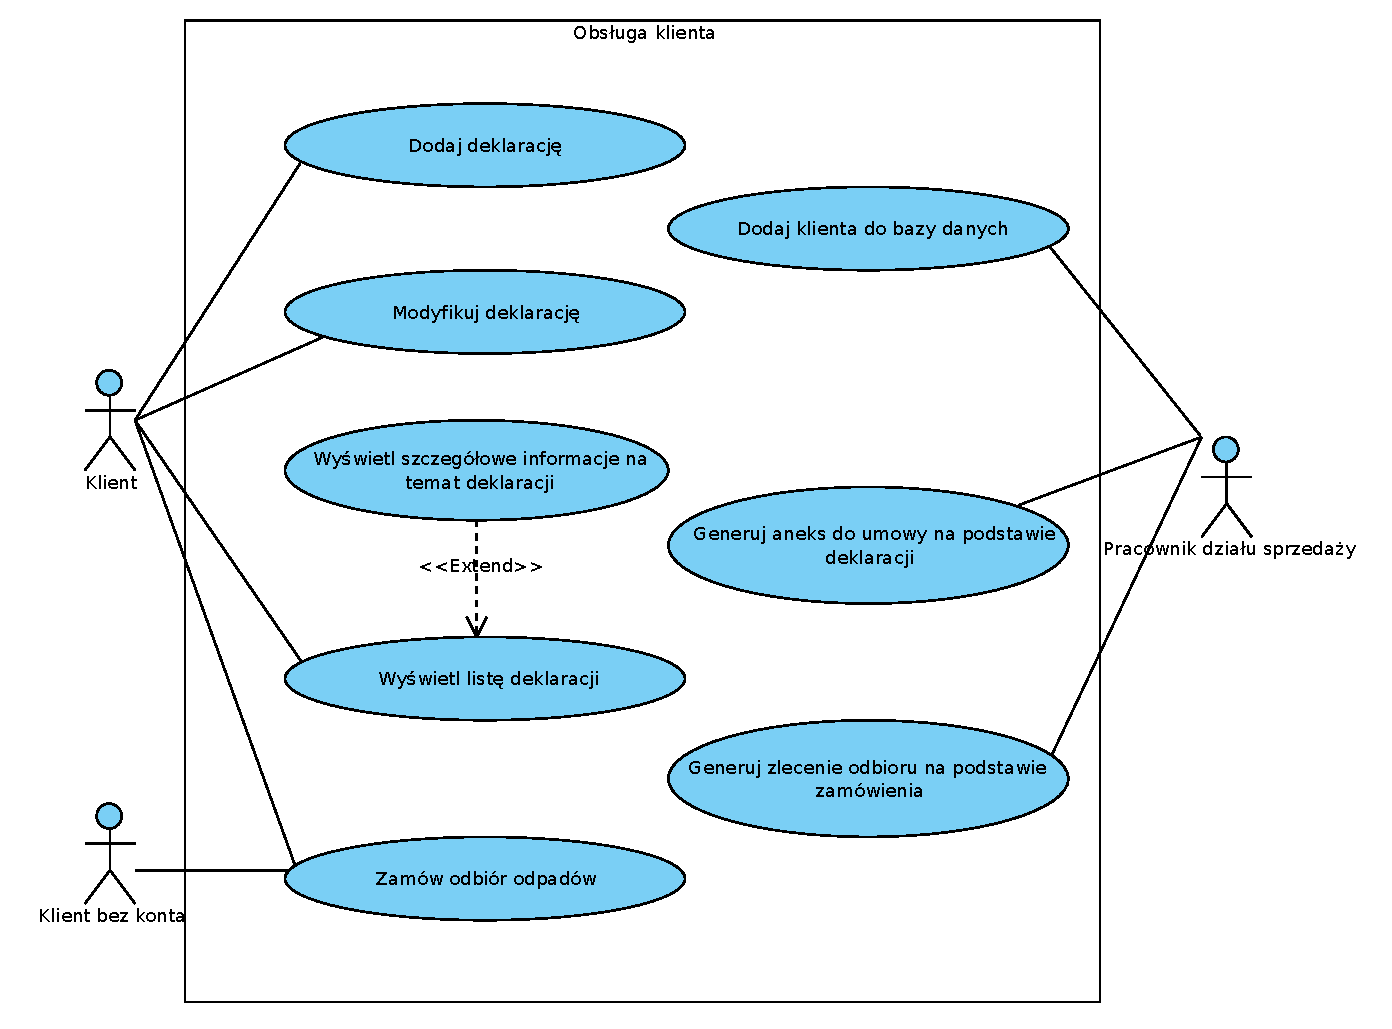
\includegraphics[width=1.1\textwidth]{img/UC/deklaracje.eps}
	\end{figure}

	\begin{usecase}{Dodaj deklarację} 
		\author{Beata Obrok}
		\goal{dodanie deklaracji}
		\context{przejęcie obowiązku odzyskania odpadów}
		\scope{System obsługi klienta}
		\actor{Klient}
		\trigger{wybranie opcji 'Dodaj deklarację'}
		\precondition{klient jest zalogowany w systemie}
		\guarantee{błędna deklaracja nie zostanie zapisana w systemie}
		\maketitle
		\begin{scenario}
			\begin{enumerate}
				\item Klient wprowadza rok, na który chce deklarować
				\extitem{it:months} Klient poprawnie wybiera miesiące, na które chce deklarować
				\item Klient wybiera kategorię odpadów z listy kategorii
				\extitem{it:list} System wyświetla listę odpadów z danej kategorii, które zostały zawarte w umowie z klientem
				\item Klient wybiera odpady, które chce zadeklarować
				\extitem{it:num} Klient poprawnie wprowadza ilości i/lub wagi wybranych odpadów
				\item Klient wybiera opcję wysłania deklaracji
				\extitem{it:verified} System pozytywnie weryfikuje poprawność deklaracji
				\item System zapisuje deklarację w systemie
				\extitem{it:saved} System wyświetla informację o poprawnym zapisaniu deklaracji w systemie
			\end{enumerate}
		\end{scenario}
		\begin{extensions}
			\begin{extlist}{it:months}{Klient wybrał miesiące, na które istnieją już deklaracje}
				\item System wyświetla informację o niemożliwości dodanie deklaracji
			\end{extlist}
			\begin{extlist}{it:list}{Klient wybiera opcję wyświetlania wszystkich odpadów}
				\item System wyświetla listę wszystkich odpadów z danej kategorii 
				\item Klient wybiera odpady, które chce zadeklarować 
				\item System wysyła informację do opiekuna klienta o potrzebie podpisania aneksu do umowy -> pt 6 
			\end{extlist}
			\begin{enumerate}
			\refitem{it:num} Klient wprowadza błędną ilość odpadów -> System wyświetla informację o błędnych danych 
			\refitem{it:verified} System negatywnie weryfikuje poprawność deklaracji -> Wyświetla informację o błędnych danych 
			\refitem{it:saved} System wyświetla informację o błędzie zapisu do bazy danych 
			\end{enumerate}
		\end{extensions}
\end{usecase}

	\begin{usecase}{Wyświetl listę deklaracji}
		\author{Beata Obrok}
		\goal{Wylistowanie deklaracji złożonych przez klienta}
		\context{chęć przejżenia deklaracji}
		\scope{System obsługi klienta}
		\actor{Klient}
		\trigger{wybranie zakładki z listą deklaracji}
		\precondition{klient jest zalogowany}
		\maketitle
		\begin{scenario}
			\begin{enumerate}
				\item System wyświetla deklaracje przypisane do nazwy użytkownika klienta
			\end{enumerate}
		\end{scenario}
\end{usecase}

	\begin{usecase}{Modyfikuj deklarację}
		\author{Beata Obrok}
		\goal{Modyfikacja dodanej przez tego klienta deklaracji}
		\context{chęć modyfikacji istniejącej deklaracji}
		\scope{System obsługi klienta}
		\actor{Klient}
		\trigger{wybranie przycisku modyfikacji wybranej deklaracji}
		\precondition{klient jest zalogowany}
		\guarantee{w przypadku błędu deklaracja pozostanie w stanie oryginalnym}
		\maketitle
		\begin{scenario}
			\begin{enumerate}
				\item System wyświetla stronę modyfikacji deklaracji
				\item System wyświetla listę odpadów z kategorii dotyczącej danej deklaracji
				\item Klient wybiera odpady, które chce zadeklarować
				\item Klient poprawnie modyfikuje ilości i/lub wagi wybranych odpadów
				\item Klient wybiera opcję wysłania deklaracji
				\item System pozytywnie weryfikuje poprawność deklaracji
				\item System zapisuje deklarację w systemie
				\item System wyświetla informację o poprawnym zapisaniu deklaracji w systemie
			\end{enumerate}
		\end{scenario}
				3.1. Klient dodaje nowe odpady do deklaracji
					\indent 4.1.1. Klient wpisuje ilości i/lub wagi wybranych odpadów -> pt 5
				3.2. Klient wybiera opcję wyświetlania wszystkich odpadów \\
					\indent 4.1.1. System wyświetla listę wszystkich odpadów z danej kategorii \\
					\indent 4.1.2. Klient wybiera odpady, które chce zadeklarować \\
					\indent 4.1.3. System wysyła informację do opiekuna klienta o potrzebie podpisania aneksu do umowy -> pt 5 \\
				4.1. Klient wprowadza błędną ilość odpadów -> System wyświetla informację o błędnych danych \\
				6.1. System negatywnie weryfikuje poprawność deklaracji -> Wyświetla informację o błędnych danych \\
				8.1. System wyświetla informację o błędzie zapisu do bazy danych \\
\end{usecase}

	\begin{usecase}{Wyświetl szczegółowe informacje na temat deklaracji}
		\author{Beata Obrok} 
		\goal{Wyświetlenie szczegółów wybranej deklaracji} 
		\context{chęć dostania szczegółowych informacji o deklaracji}
		\scope{System obsługi klienta} 
		\level{biznesowy} 
		\actor{Klient} 
		\trigger{wybranie deklaracji z listy deklaracji użytkownika} 
		\precondition{klient jest zalogowany i ma wyświetloną listę deklaracji} 
		\maketitle
\begin{scenario}
			\begin{enumerate}
				\item System wyświetla szczegółowe informacje dotyczące danej deklaracji
			\end{enumerate}
\end{scenario}
\end{usecase}

	

	\begin{usecase}{Zleć odbiór odpadów}
		\author{Dawid Suder}
		\goal{Zlecenie odbioru odpadów od klienta}
		\context{klient chce zlecić odbiór odpadów, które chce oddać}
		\scope{System obsługi klienta}
		\actor{Klient}
		\trigger{kliknięcie na stronie opcji "Zlecenie odbioru odpadów"}
		\precondition{Klient ma otwartą stronę internetową}
		\maketitle
		\begin{scenario}
			\begin{enumerate}
				\item Klient zgłasza odpady (typ, ilość/waga) do odbioru
				\item Klient wybiera opcję zapisania zlecenia
				\extitem{it:verifyzoo} System pozytywnie weryfikuje poprawność danych
				\extitem{it:savedzoo} Klient dostaje potwierdzenie przyjęcia zlecenia
			\end{enumerate}
		\end{scenario}
		\begin{extensions}
			\begin{enumerate}
				\refitem{it:verifyzoo} System negatywnie weryfikuje dane i wyświetla informację o błędzie
				\refitem{it:savedzoo} Klient dostaje informacje o błędzie w zleceniu
			\end{enumerate}
		\end{extensions}
\end{usecase}

	\begin{usecase}{Zamów surowce}
		\author{Dawid Suder}
		\goal{Zamówienie surowców przez Klienta}
		\context{Klient chce zamówić surowce w firmie}
		\scope{System obsługi klienta}
		\actor{Klient}
		\trigger{kliknięcie na stronie opcji "Zamów Surowce"}
		\precondition{Klient ma otwartą stronę internetową}
		\maketitle
		\begin{scenario}
			\begin{enumerate}
				\item Klient wybiera surowce z listy możliwych surowców
				\item Klient wprowadza ilość/wagę surowców, które wybrał
				\item Klient wybiera opcję zapisania danego zamówienia
				\extitem{it:savedzs} Klient dostaje informację o przyjęciu zamówienia
			\end{enumerate}
		\end{scenario}
		\begin{extensions}
			\begin{enumerate}
				\refitem{it:savedzs} Klient dostaje informację o niepowodzeniu w przyjęciu zamówienia
			\end{enumerate}
		\end{extensions}
\end{usecase}

	\begin{usecase}{Dodaj klienta do bazy danych}
		\author{Dawid Suder}
		\goal{Dodanie nowego klienta do istniejącej bazy danych}
		\context{chęć dodania nowego klienta przez Pracownika do bazy danych}
		\scope{System obsługi klienta}
		\actor{Pracownik działu sprzedaży}
		\trigger{Pracownik wybiera opcję dodania klienta z panelu pracowniczego}
		\precondition{Pracownik jest zalogowany do systemu i posiada dane Klienta (Umowa, Aneks)}
		\guarantee{Dane Klienta zostaną zapamiętane i będą oczekiwać na zapis do bazy}
		\maketitle
		\begin{scenario}
			\begin{enumerate}
				\item Pracownik wprowadza dane z Umowy do formularza
				\item Pracownik zapisuje Klienta do bazy
				\item System sprawdza wprowadzone dane
				\extitem{it:savedkdb} System wyświetla informację o pomyślnym zapisie
				\item Klient automatycznie dostaje wygenerowany Login i Hasło na maila z formularza
			\end{enumerate}
		\end{scenario}
		\begin{extensions}
			\begin{enumerate}
				\refitem{it:savedkdb} System wyświetla informację o błedzie w danych
			\end{enumerate}
		\end{extensions}
\end{usecase}

	\begin{usecase}{Generuj aneks do umowy na podstawie deklaracji}
		\author{Dawid Suder}
		\goal{Wygenerowanie aneksu do wybranej umowy na podstawie deklaracji}
		\context{chęć dostania aneksu do umowy}
		\scope{System obsługi Klienta}
		\actor{Pracownik działu sprzedaży}
		\trigger{Pracownik klika w przycisk "Generuj aneks"}
		\precondition{Pracownik jest zalogowany i ma wybraną umowę}
		\maketitle
		\begin{scenario}
			\begin{enumerate}
				\extitem{it:gad} System generuje aneks na podstawie umowy
			\end{enumerate}
		\end{scenario}
		\begin{extensions}
			\begin{enumerate}
			\refitem{it:gad} System wyświetla informacje o niepomyślnej generacji
			\end{enumerate}
		\end{extensions}
\end{usecase}

	\begin{figure}[H]
		\centering
		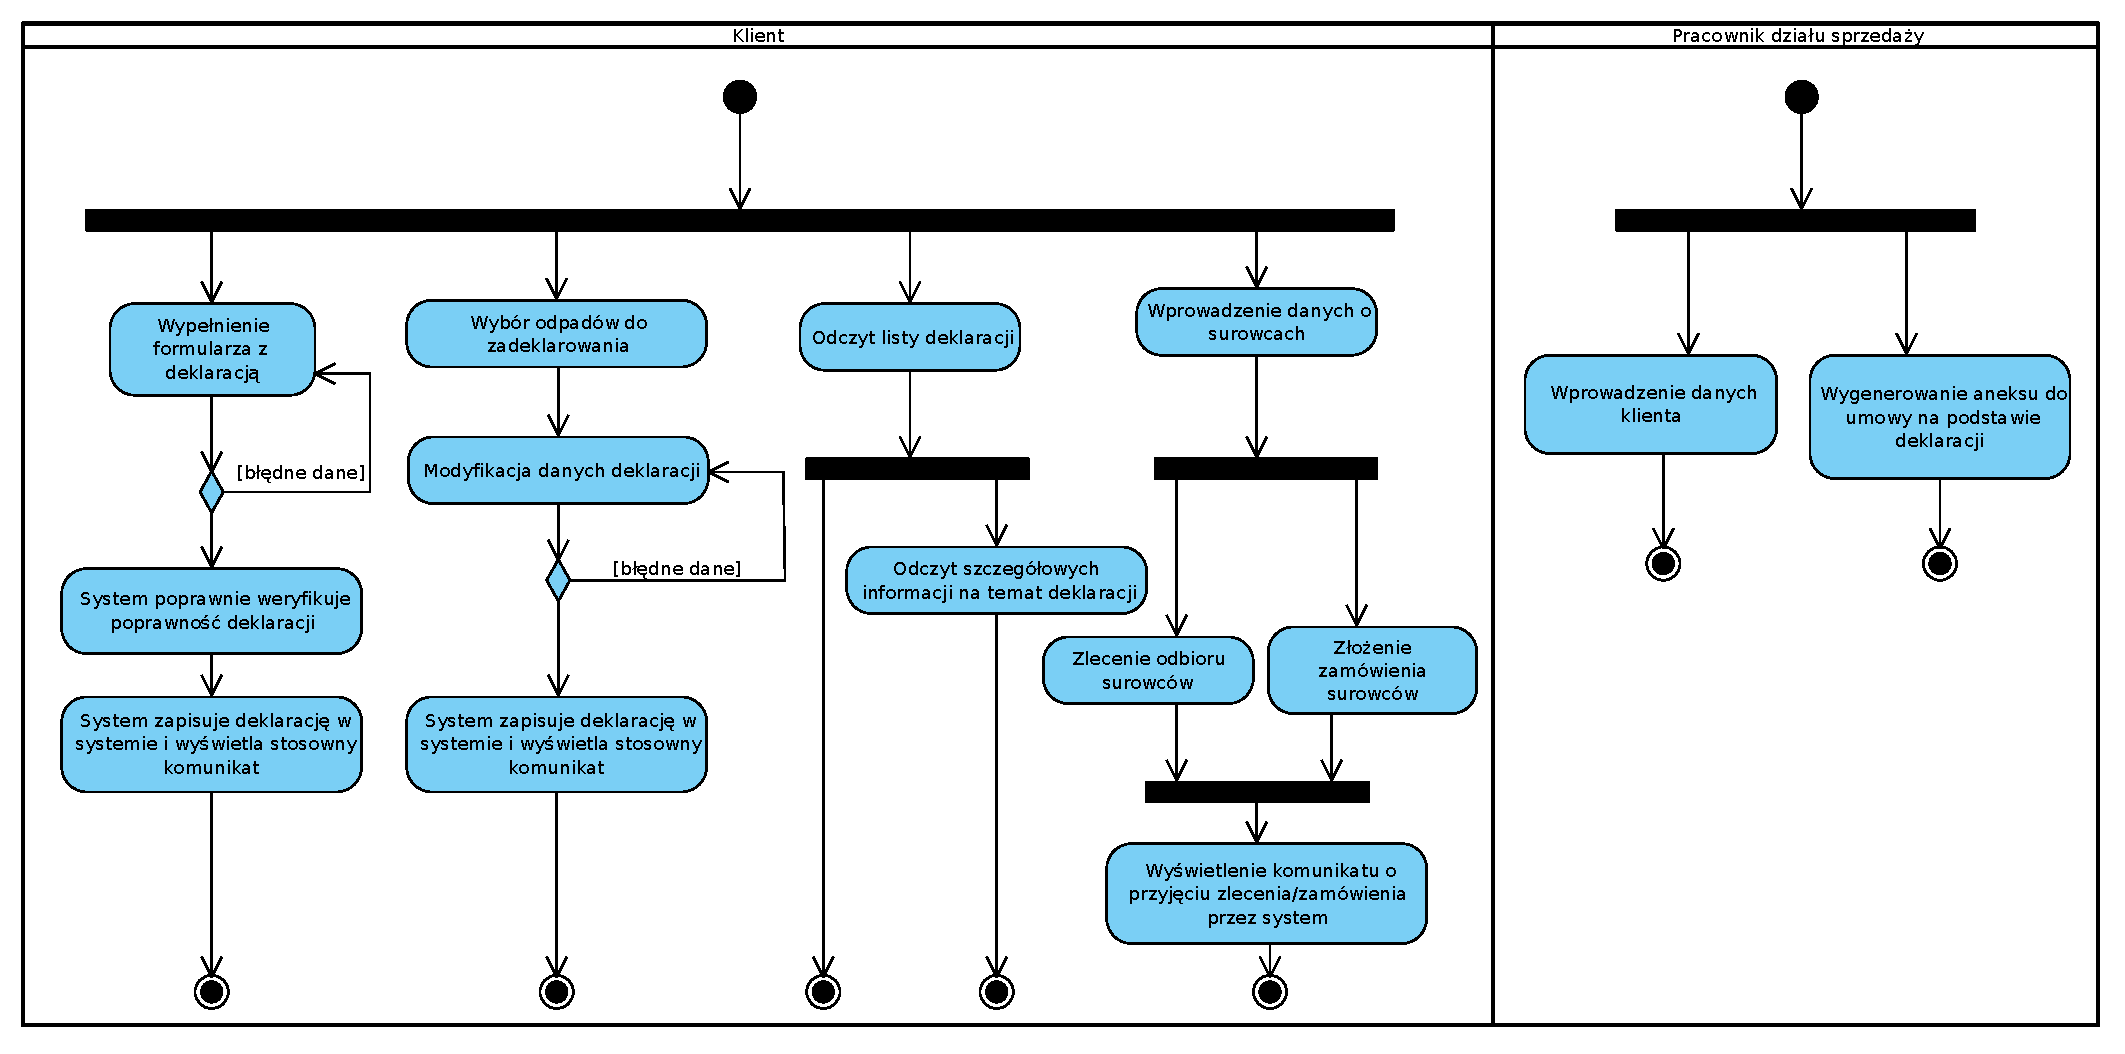
\includegraphics[width=.9\textwidth]{img/AD/klient.eps}
		\caption{Diagram aktywności dla obsługi klienta}
	\end{figure}

\subsubsection{Obsługa skupu}

	\begin{figure}[H]
		\centering
		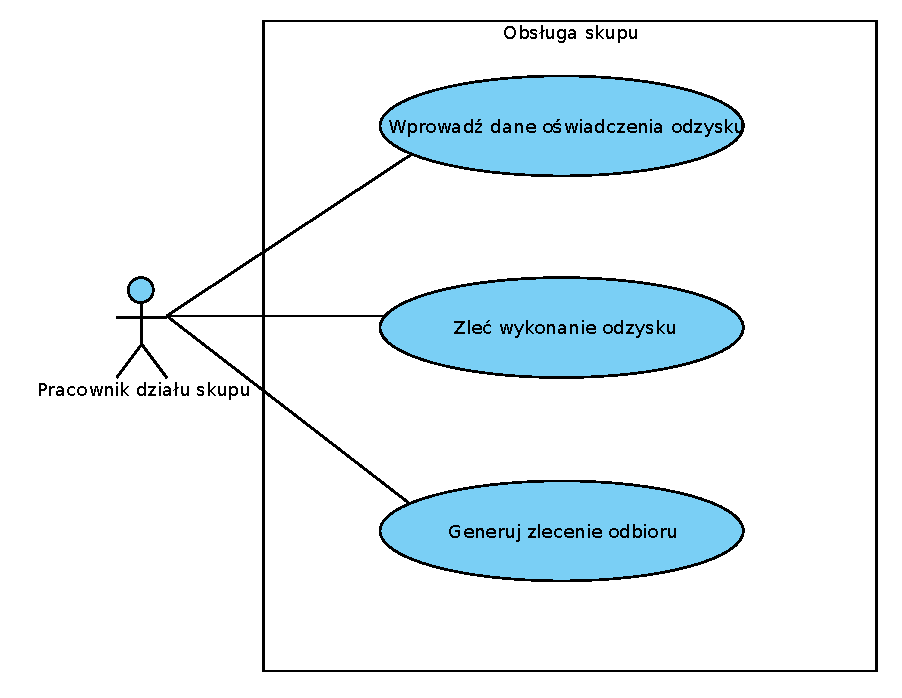
\includegraphics[width=.8\textwidth]{img/UC/skup.eps}
	\end{figure}

	\begin{usecase}{Wprowadź dane oświadczenia odzysku}
	\author{Dawid Suder} 
	\goal{Wprowadzenie oświadczenia odzysku od Zakładu przetwarzania odpadów} 
	\context{konieczność gromadzenia oświadczeń odzysku związane z Ustawą o Odzysku} 
	\scope{System obsługi skupu} 
	\level{biznesowy} 
	\actor{Pracownik działu skupu} 
	\trigger{Otrzymanie oświadczenia odzysku} 
	\precondition{pracownik wysłał zlecenie przetworzenia odpadów } 
	\guarantee{w przypadku niepoprawności danych oświadczenia nie zostanie dodane do bazy} 
	\maketitle
\begin{scenario} 
		\begin{enumerate}
			\item Pracownik pozytywnie weryfikuje oświadczenie na podstawie deklaracji i zlecenia
			\item Pracownik zapisuje dane oświadczenia odzysku
		\end{enumerate}
	\end{scenario}
\begin{extensions}
			1.1. Pracownik negatywnie weryfikuje dane w oświadczeniu -> wysyła informację do Zakładu
	\end{extensions}
\end{usecase}

	\begin{usecase}{Zleć wykonanie odzysku}
		\author{Dawid Suder} 
		\goal{Zlecenie wykonania odzysku Zakładom przetwarzania odpadów} 
		\context{konieczność zlecania wykonania odzysku w celu uzyskania oświadczeń} 
		\scope{System obsługi skupu} 
		\level{biznesowy} 
		\actor{Pracownik działu skupu} 
		\trigger{Otrzymanie deklaracji} 
		\precondition{pracownik otrzymał deklarację dla której potrzebne jest oświadczenie } 
		\guarantee{w przypadku przeoczenia deklaracji istnieje możliwość utworzenia zlecenia grupowego} 
		\maketitle
\begin{scenario} 
			\begin{enumerate}
				\item Pracownik otrzymuje powiadomienie o nowej deklaracji
				\item Pracownik wybiera Zakład przetwarzania odpadów
				\item Pracownik tworzy dla tego zakładu zlecenie przetworzenia odpadów
			\end{enumerate}
		\end{scenario}
\begin{extensions}
				1.1. Pracownik dostaje wiele deklaracji i grupuje je w jedno zlecenie
	\end{extensions}
\end{usecase}

	\begin{usecase}{Generuj zlecenie odbioru na podstawie oferty sprzedaży}
		\author{Beata Obrok} 
		\goal{Wysłanie kierowcy do klienta w celu odbioru odpadów} 
		\context{konieczność weryfikacji danych oferty oraz przydzielenia kierowcy do zlecenia} 
		\scope{System obsługi skupu} 
		\level{biznesowy} 
		\actor{Pracownik działu skupu} 
		\trigger{wybór oferty i wybranie opcji generowania zlecenia} 
		\precondition{pracownik ma uprawnienia do dodawania zleceń } 
		\guarantee{w przypadku niepoprawności danych oferty zlecenie nie zostanie wygenerowane} 
		\maketitle
\begin{scenario} 
			\begin{enumerate}
				\item Pracownik pozytywnie weryfikuje możliwość wykonania zlecenia
				\item Pracownik zapisuje dane zamawiającego w systemie
				\item Pracownik przydziela kierowcę do zlecenia
				\item Pracownik zapisuje zlecenie w systemie
			\end{enumerate}
		\end{scenario}
\begin{extensions}
				1.1. Pracownik negatywnie weryfikuje możliwość wykonania zlecenia -> wysyła informację do klienta
	\end{extensions}
\end{usecase}

	\begin{figure}[H]
		\centering
		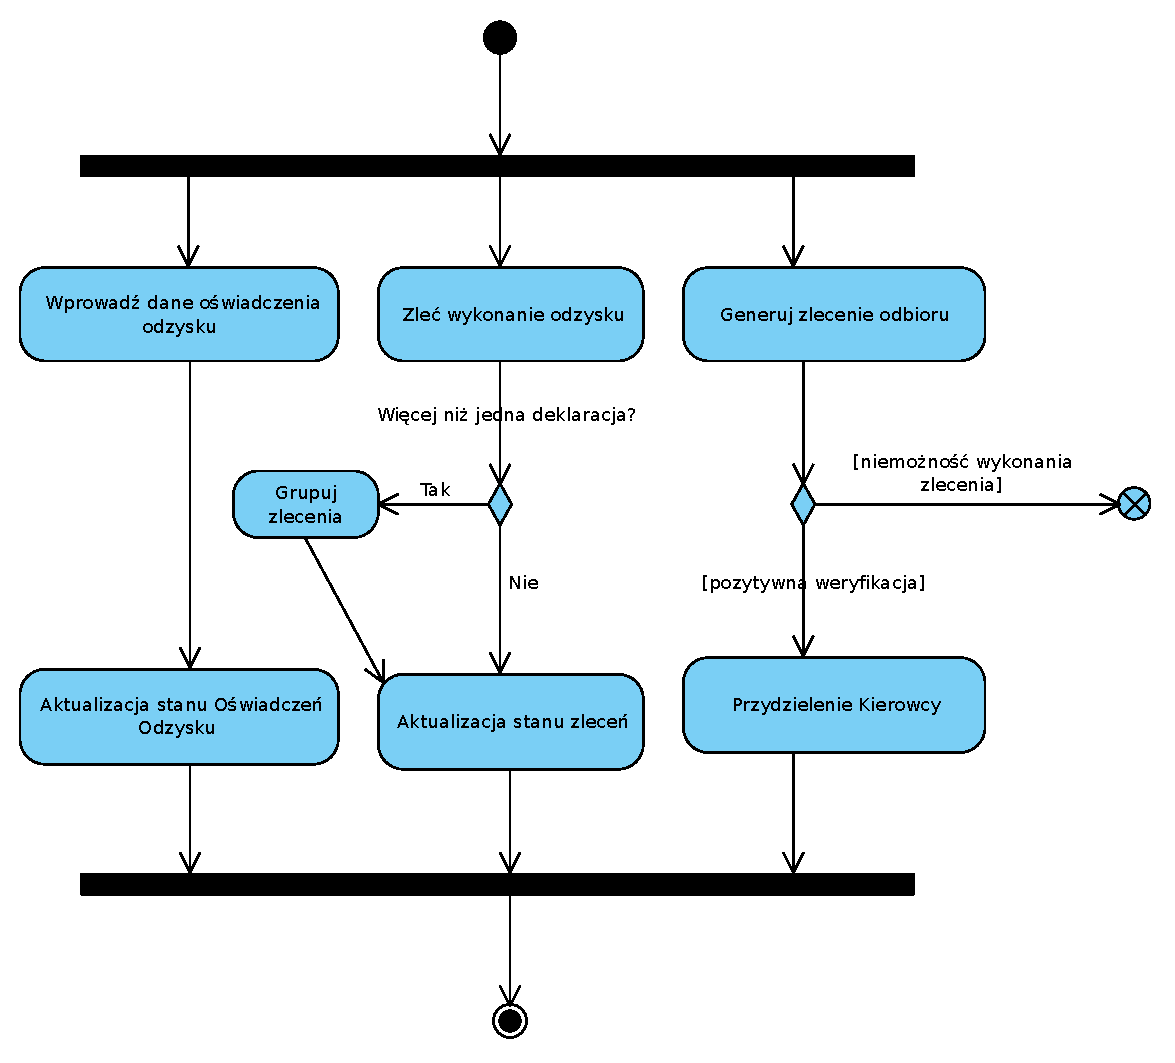
\includegraphics[width=.9\textwidth]{img/AD/skup.eps}
		\caption{Diagram aktywności dla obsługi magazynu}
	\end{figure}

\subsubsection{Obsługa księgowości}
	\begin{figure}[H]
		\centering
		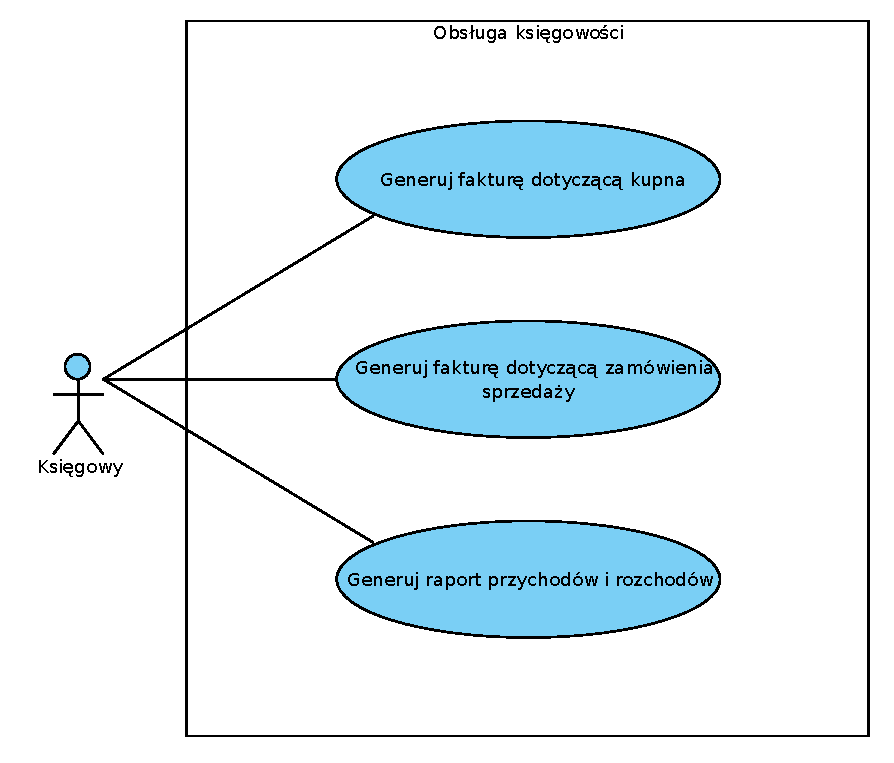
\includegraphics[width=\textwidth]{img/UC/ksiegowosc.eps}
	\end{figure}

	\begin{usecase}{Generuj fakturę sprzedaży produktów recyklingu}
		\author{Arkadiusz Socha} 
		\goal{Wygnerowanie faktury} 
		\context{otrzymanie dokumentu dowodu sprzedaży produktów } 
		\scope{system księgujący} 
		\level{biznesowy} 
		\actor{Księgowy} 
		\trigger{sprzedaż produktów recyklingu} 
		\precondition{księgowy posiada identyfikator zamówienia } 
		\guarantee{w przypadku, gdy nie będzie można wygenerować faktury, system poinformuje o tym aktora, nie generując błędnego dokumentu} 
		\maketitle
\begin{scenario}
 
			\begin{enumerate}
				\item Księgowy wybiera z listy zamówienie
				\item System upewnie się, czy o to zamówienie chodzi
				\item System generuje fakturę 
			\end{enumerate}
\end{scenario}
\end{usecase}

	\begin{usecase}{Generuj fakturę dotyczącą usługi przejęcia obowiązku recyklingu}
		\author{Arkadiusz Socha} 
		\goal{Wygnerowanie faktury} 
		\context{otrzymanie dokumentu dowodu zakupu oświadczenia } 
		\scope{system księgujący} 
		\level{biznesowy} 
		\actor{Księgowy} 
		\trigger{kupno oświadczenia oddzysku} 
		\precondition{księgowy posiada identyfikator danych dotyczących odpowiedniej oferty sprzedaży } 
		\guarantee{w przypadku, gdy nie będzie można wygenerować faktury, system poinformuje o tym aktora, nie generując błędnego dokumentu} 
		\maketitle
\begin{scenario}
 
			\begin{enumerate}
				\item Księgowy wybiera z listy ofertę sprzedaży
				\item System upewnie się, czy o tą ofertę chodziło
				\item System generuje fakturę 
			\end{enumerate}

\end{scenario}
\end{usecase}

	\begin{usecase}{Wprowadź dane faktury kupna oświadzczenia odzysku}
		\author{Arkadiusz Socha} 
		\goal{Wpisanie do systemu danych o fakturze} 
		\context{posiadanie w bazie wszystkich informacji o operacjach firmy}
		\scope{system księgujący} 
		\level{biznesowy} 
		\actor{Księgowy} 
		\trigger{kupno oświadczenia oddzysku} 
		\precondition{księgowy posiada dane o fakturze kupna oświadczenia o przetworzeniu odpadów } 
		\guarantee{w przypadku, gdy nie będzie można wproawdzić danych do bazy, nie zostanie ona zmodyfikowana} 
		\maketitle
\begin{scenario}
 
			\begin{enumerate}
				\item Księgowy wpisuje dane z faktury do wygenerowanego formularza
				\item System sprawdza czy format poszczególnych danych jest prawidłowy
				\item System wprowadza dane do systemu
			\end{enumerate}
		\end{scenario}
\begin{extensions}
		2.1 Jeżeli jakieś dane są niepoprawne, księgowy zostaje o tym poinformowany i musi wprowadzić je ponownie
	\end{extensions}
\end{usecase}

	\begin{usecase}{Generuj raport przychodów i rozchodów}
		\author{Arkadiusz Socha} 
		\goal{Wygnerowanie raportu o zyskach i stratach firmy} 
		\context{otrzymanie raportu dla właściciela } 
		\scope{system księgujący} 
		\level{biznesowy} 
		\actor{Właściciel} 
		\trigger{właściciel chce mieć informację o przychodach i rozchodach firmy w danym okresie czasowym} 
		\precondition{podanie ram czasowych  } 
		\guarantee{w przypadku, gdy nie będzie można wygenerować raportu, system poinformuje o tym właściciela, nie generując błędnych informacji} 
		\maketitle
\begin{scenario}
 
			\begin{enumerate}
				\item Właściciel podaje ramy czasowe okresu, ktory go interesuje
				\item System wybiera tylko te faktury, które zawierają się w podanym przedziale czasowym
				\item System generuje raport
			\end{enumerate}
		\end{scenario}
\begin{extensions}
		1.1 Ramy czasowe są błędne - conajmniej jedna z wartości jest w przyszłości, system wygeneruje błąd i poprosi o ich ponowne wpisanie
	\end{extensions}
\end{usecase}

	\begin{figure}[H]
		\centering
		\centerline{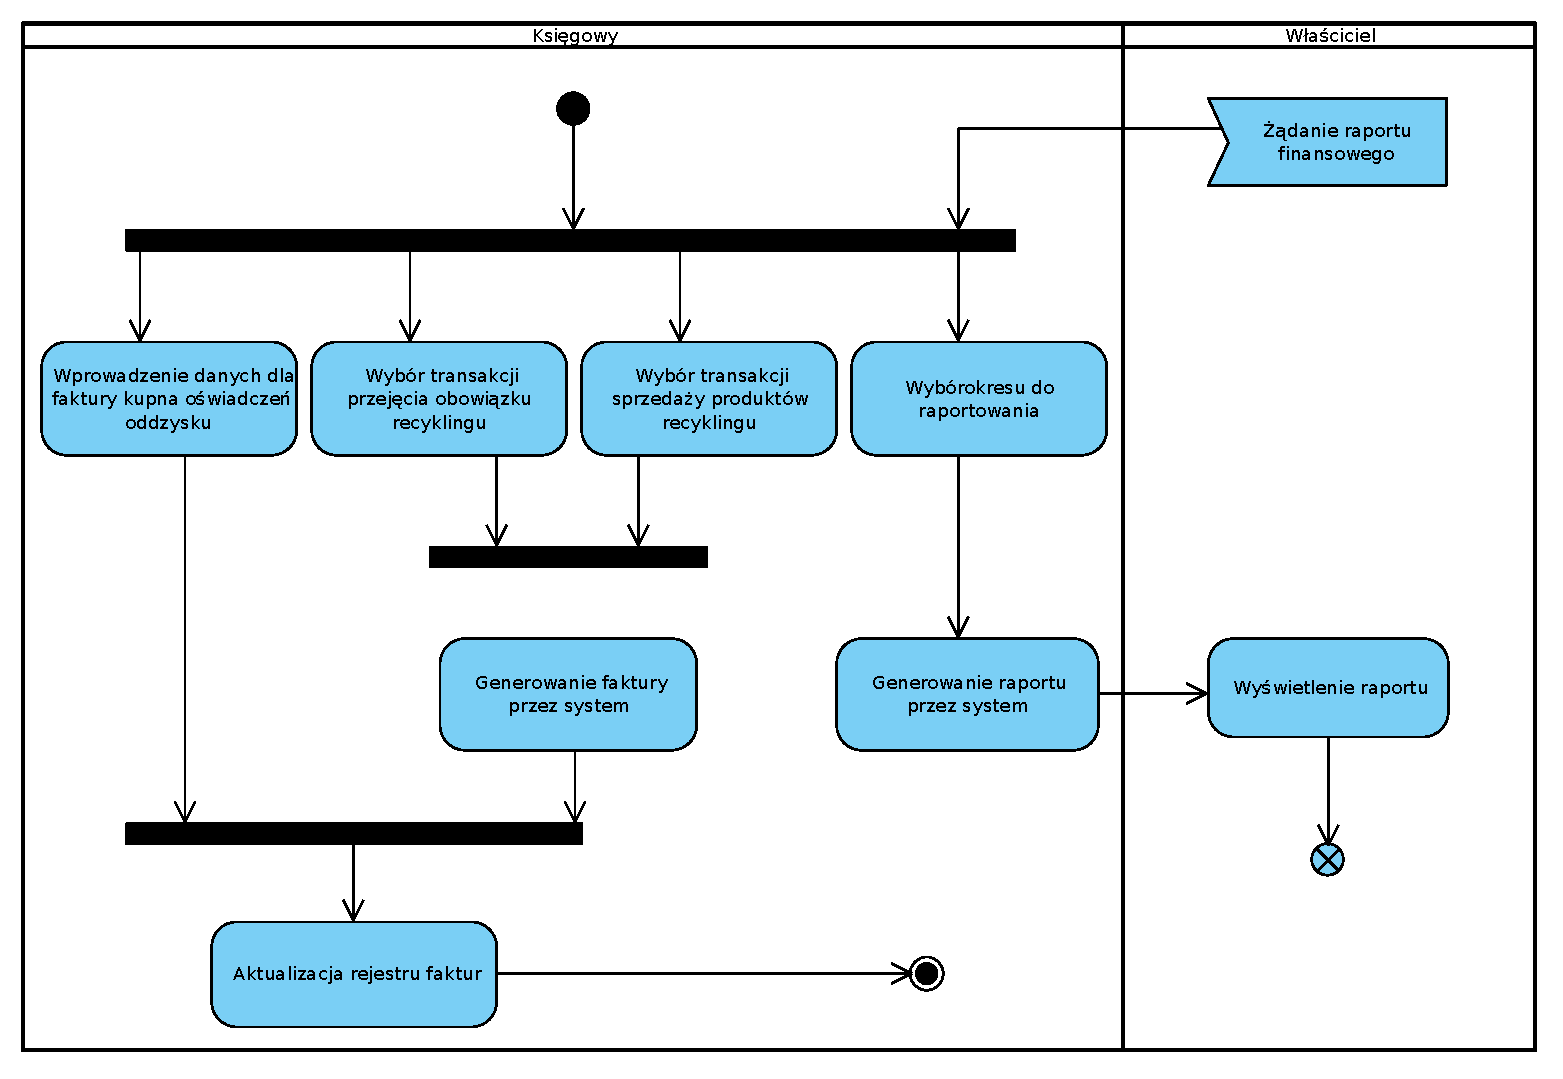
\includegraphics[width=1.2\textwidth]{img/AD/ksiegowosc.eps}}
		\caption{Diagram aktywności dla obsługi księgowości}
	\end{figure}

\subsubsection{Obsługa magazynu}

	\begin{figure}[H]
		\centering
		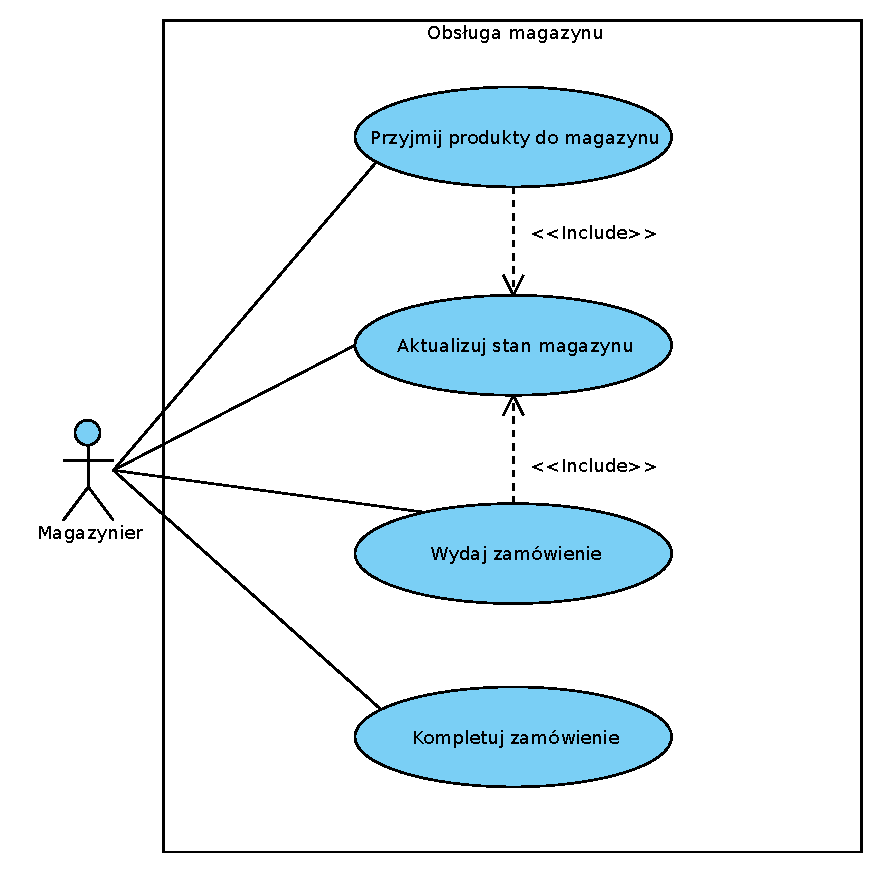
\includegraphics[width=.8\textwidth]{img/UC/magazyn.eps}
	\end{figure}

	\begin{usecase}{Przyjmij produkty do magazynu}
		\author{Arkadiusz Socha} 
		\goal{Dodanie produktów recyklingu do magazynu i aktualizacja stanu magazynu} 
		\context{przechowanie produktów recyklingu w magazynie}
		\scope{system magazynowy} 
		\level{biznesowy} 
		\actor{Magazynier} 
		\trigger{dostarczenie przez kierowce produktów do magazynu} 
		\precondition{kierowca ma produkty recyklingu, które należy zmagazynować oraz ich listę } 
		\guarantee{w przypadku, gdy produkty nie zostaną zmagazynowane, stan magazynu nie będzie zmieniany} 
		\maketitle
\begin{scenario} 
			\begin{enumerate}
				\item Kierowca przywozi produkty
				\item Magazynier układa je w magazynie
				\item Magazynier aktualizuje stan magazynu
			\end{enumerate}
\end{scenario}
\end{usecase}

	\begin{usecase}{Wydaj zamówienie}
		\author{Arkadiusz Socha} 
		\goal{Wydanie kierowcy produktów, ujętych w zamówieniu} 
		\context{potrzeba przetransporotowania produktów do kupca}
		\scope{system magazynowy} 
		\level{biznesowy} 
		\actor{Magazynier} 
		\trigger{przyjazd kierowcy do magazynu} 
		\precondition{kierowca ma zamówienie } 
		\guarantee{w przypadku, gdy nie można skompletować zamówienia stan magazynu się nie zmieni} 
		\maketitle
\begin{scenario}
 
			\begin{enumerate}
				\item Kierowca przekazuje numer zamówienia magazynierowi
				\item Magazynier wydaje produkty kierowcy
				\item Magazynier uaktualnia stan magazynu
			\end{enumerate}
		\end{scenario}
\begin{extensions}
		1.1 W przypadku gdy magazynier nie otrzymał wcześniej informacji o zamówieniu, kompletuje je teraz, w razie niepowodzenia produkty nie zostają wydane\\
	\end{extensions}
\end{usecase}

	\begin{usecase}{Aktualizuj stan magazynu}
		\author{Arkadiusz Socha} 
		\goal{Aktualizacja danych o stanie magayznu} 
		\context{utrzymywanie aktualnej informacji o ilości produktów w magazynie} 
		\scope{system magazynowy} 
		\level{użytkowy} 
		\actor{Magazynier} 
		\trigger{wydanie lub przyjęcie produktów} 
		\precondition{zmiana stanu magazynu } 
		\guarantee{w przypadku, gdy nie można zaktualizować stanu magazynu, jego stan pozostanie niezmieniony} 
		\maketitle
\begin{scenario}
 
			\begin{enumerate}
				\item Magazynier wpisuje informację o wydanych/przyjętych produktach do wygenerowanego formularza
				\item System sprawdza poprawność danych(np. czy magazynier nie wydał więcej niż było w magazynie)
				\item System aktualizje dane
			\end{enumerate}
		\end{scenario}
\begin{extensions}
		2.1 W przypadku błędnych danych, system informuje o tym magazyniera i prosi o ich ponowne wpisanie\\
	\end{extensions}
\end{usecase}

	\begin{usecase}{Kompletuj zamówienie}
		\author{Arkadiusz Socha} 
		\goal{Skompletowanie zamówienie w celu wydania go kierowcy} 
		\context{chęć uporządkowania produktów do zamówienia w celu szybkiego ich przekazania kierowcy} 
		\scope{system magazynowy} 
		\level{biznesowy} 
		\actor{Magazynier} 
		\trigger{dostanie informacji o zamówieniu} 
		\precondition{odpowiednia ilość towarów w magazynie } 
		\guarantee{w przypadku, gdy nie ma odpowiedniej ilości towarów w magazynie, zostanie wysłana informacja zwrotna } 
		\maketitle
\begin{scenario}
 
			\begin{enumerate}
				\item Magazynier otrzymuje listę towarów, które wchodzą w skład zamówienia
				\item Magazynier sprawdza czy posiada ich odpowiednią ilość
				\item Magazynier przygotowuje zamówienie
			\end{enumerate}
		\end{scenario}
\begin{extensions}
		2.2. Nie można skompletować zamówienia, zostaje wysłana informacja zwrotna o nieposiadanych towarach\\
	\end{extensions}
\end{usecase}

	\begin{figure}[H]
		\centering
		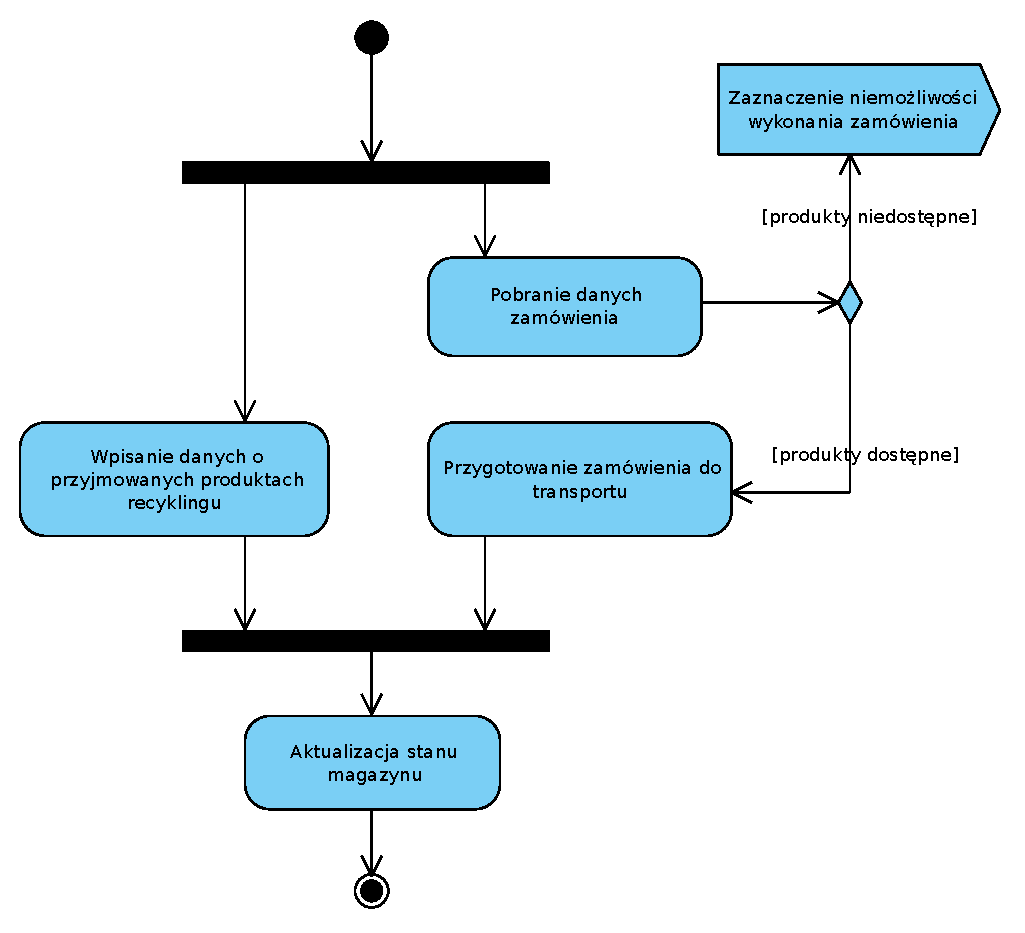
\includegraphics[width=.9\textwidth]{img/AD/magazyn.eps}
		\caption{Diagram aktywności dla obsługi magazynu}
	\end{figure}

\subsubsection{Obsługa kierowców}

	\begin{figure}[H]
		\centering
		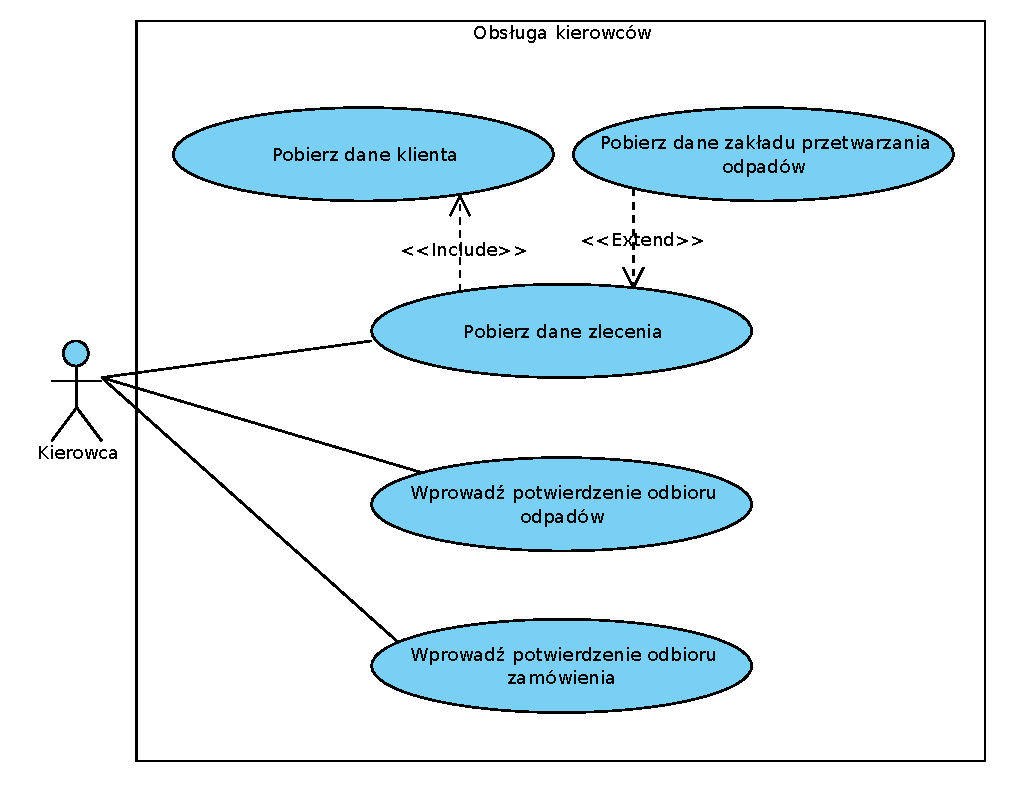
\includegraphics[width=.8\textwidth]{img/UC/kierowcy.eps}
	\end{figure}

	\begin{usecase}{Pobierz dane zlecenia}
		\author{Dawid Suder}
		\goal{Pobranie szczegółów wybranego zlecenia}
		\context{Kierowca chce dostać szczegóły dotyczące zlecenia}
		\scope{Obsługa kierowców}
		\actor{Kierowca}
		\trigger{Kierowca naciska przycisk Wyświetl Szczegóły w zleceniu}
		\precondition{Kierowca jest zalogowany do Systemu}
		\maketitle
		\begin{scenario}
			\begin{enumerate}
				\extitem{it:datapdz} System wyświetla szczegóły zlecenia
			\end{enumerate}
		\end{scenario}
		\begin{extensions}
			\begin{enumerate}
			\refitem{it:datapdz} System wyświetla informację o niemożliwości wyświetlenia szczegółów
			\end{enumerate}
		\end{extensions}
\end{usecase}

	\begin{usecase}{Wprowadź potwierdzenie odbioru odpadów}
		\author{Dawid Suder}
		\goal{Potwierdzenie odbioru odpadów od Klienta}
		\context{Kierowca chce potwierdzić odbiór}
		\scope{Obsługa kierowców}
		\actor{Kierowca}
		\trigger{Kierowca wybiera odpowiednią opcję w panelu Kierowcy}
		\precondition{Kierowca jest zalogowany}
		\maketitle
		\begin{scenario}
			\begin{enumerate}
				\extitem{it:pook} Kierowca potwierdza dane ze zlecenia
				\item System wyświetla informację o pomyślnej zmianie stanu zlecenia
			\end{enumerate}
		\end{scenario}
		\begin{extensions}
			\begin{enumerate}
			\refitem{it:pook} Kierowca poprawia zlecenie na rzeczywiste dane
			\end{enumerate}
		\end{extensions}
\end{usecase}

	\begin{usecase}{Wprowadź potwierdzenie odbioru zamówienia}
		\author{Dawid Suder}
		\goal{Wprowadzenie potwierdzenia odbioru do systemu w celu zaznaczenia wykonania zamówienia}
		\context{Kierowca chce zaznaczyć wykonanie odbioru zamówienia}
		\scope{Obsługa kierowców}
		\actor{Kierowca}
		\trigger{Kierowca zaznacza opcję Potwierdzenia odbioru w panelu kierowcy dla danego zamówienia}
		\precondition{Kierowca jest zalogowany w systemie}
		\guarantee{Zamówienie pozostanie nie zmienione}
		\maketitle
		\begin{scenario}
			\begin{enumerate}
				\extitem{it:wpo} System wyświetla informację o zmianie statusu zamówienia
			\end{enumerate}
		\end{scenario}
		\begin{extensions}
			\begin{enumerate}
				\refitem{it:wpo} System wyświetla informację o błędzie
			\end{enumerate}
		\end{extensions}
\end{usecase}


	\begin{figure}[H]
		\centering
		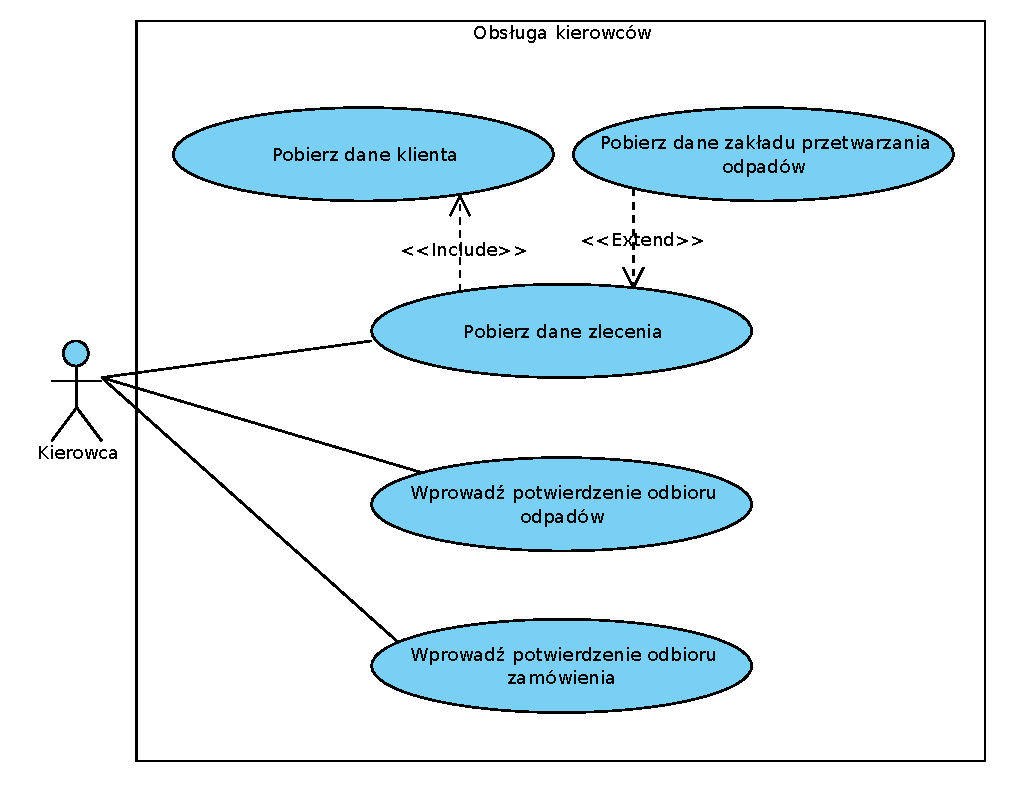
\includegraphics[width=.8\textwidth]{img/UC/kierowcy.eps}
	\end{figure}
